\section{Программа генератора}
\subsection{Обзор и установка}
Генератор находится в стадии прототипа и не встроен в игру, поэтому на данный момент представляет собой отдельную программу с графическим интерфейсом. Внешний вид программы генератора после запуска представлен ниже:

\begin{figure}[H]
\center
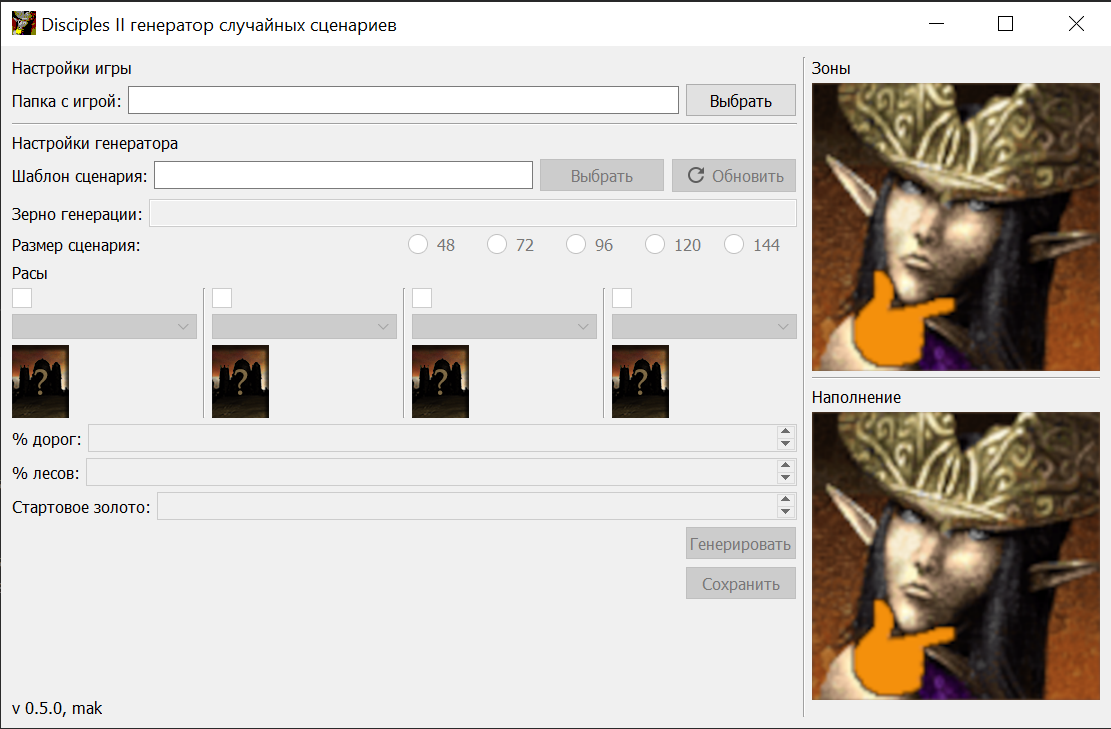
\includegraphics[width=.8\linewidth]{docImages/interface.png}
\caption{Интерфейс программы генератора}
\end{figure}

Генератор не привязан к конкретному моду и, при наличии корректного файла настроек, может работать как с оригинальной Disciples II: Rise of the Elves (v 3.01), так и с любыми модами.

Прототип генератора \textbf{не нуждается} в тулсете для моддинга \href{https://github.com/VladimirMakeev/D2ModdingToolset}{\texttt{mss32.dll}} и работает независимо от его наличия.
Для того чтобы генератор мог корректно создавать сценарии ему необходим файл с настройками \texttt{generatorSettings.lua}, который должен быть помещен в папку \texttt{Scripts} внутри папки с игрой.\\
В данном файле задаются \qq{подсказки} для генератора - информация об игре, которую невозможно определить алгоритмически:
\begin{itemize}
\item списки юнитов и предметов, запрещенных к использованию генератором
\item списки изображений магазинов, башен магов, лагерей наемников, тренеров и руин. Их наземные и водные варианты
\item списки лендмарок (Landmarks) наиболее подходящих визуально для расположения на территориях игровых рас, нейтральной территории, а также выглядящих как горы
\end{itemize}

Данный подход позволяет генератору не зависеть от особенностей модификации игры, но давая возможность настроить баланс и визуальную части генерации ценой одного дополнительного файла на языке \href{https://www.lua.org/}{Lua}.

Вместе с программой генератором и этой документацией идут заранее подготовленные файлы настроек \texttt{generatorSettings.lua} для PvP-модов \href{https://norvezskayasemga.pro/}{sMNS (v1.0.1.2+)} и \href{https://drive.google.com/drive/folders/1RKBPSrk6SC4viXzhdPFkUHgwEqOl3WeT}{Мотлина (v 1.5.3+)}. Перед использованием генератора файлы настроек, как было сказано ранее, необходимо закинуть в папку \texttt{Scripts} внутри папки с игрой.

\newpage
\subsection{Генерация сценария по шаблону}
Интерфейс программы сделан с целью минимизации ошибок со стороны пользователя во время использования. Недоступные в данный момент кнопки и элементы становятся неактивными и активируются когда их использование возможно.\\
Типичный вариант использования программы:
\begin{itemize}
\item Выбор папки с игрой. В верхней части интерфейс в строке \texttt{"Папка с игрой"} необходимо нажать кнопку \texttt{"Выбрать"} и выбрать \textbf{папку} игры
\item Если файл настроек генератора был заранее добавлен в папку \texttt{Scripts} внутри папки игры, должна стать доступна опция выбора шаблона сценария напротив строки \texttt{"Шаблон сценария"}
\item После выбора шаблона станет доступна кнопка \texttt{"Обновить"}, она будет полезна при разработке и тестировании шаблона. См. \hyperref[templateDevelopment]{\selectlanguage{Russian}Разработка шаблона} 
\item После выбора шаблона будут доступны опции влияющие на создаваемый сценарий. Они будут подробно рассмотрены далее
\item Также, внизу станет доступна кнопка \texttt{"Генерировать"}, которая запустит сам процесс генерации с учетом содержимого шаблона и выбранных пользователем опций генерации
\item Во время генерации интерфейс станет неактивен во избежание смены настроек посреди процесса генерации
\item По окончании генерации интерфейс снова станет активен, а также станет доступна кнопка \texttt{"Сохранить"} для записи результатов генерации в файл сценария \texttt{(.sg)} на жестком диске.
\item Для удобства пользователей и авторов шаблонов справа в окне программы находятся две области предпросмотра: просмотр расположения зон и "миникарта" с данными об их наполнении. Области автоматически обновляются после каждой успешной генерации сценария
\end{itemize}

\newpage
\subsection{Опции генерации}
\label{templateOptions}
Опции генерации сценария представляют собой те настройки шаблона, которые автор разрешил пользователям менять. Таким образом значения по умолчанию и некоторые параметры целиком зависят от шаблона. Программа генератора лишь выводит их в интерфейс для удобства выбора пользователем.
Опции генерации сценария:\\
\begin{itemize}
\item Зерно генерации - целое число определяющее зерно для генератора случайных чисел, используемого при создании сценария. \textbf{Важно:} генератор обладает свойством воспроизводимости. При использовании одинаковой версии генератора, мода и его версии, шаблона, зерна генерации, размера сценария, списка рас, \% дорог и лесов результаты генерации будут полностью идентичны и воспроизводимы
\item Размер сценария - размер игровой карты в тайлах. Доступные для выбора пользователя размеры зависят от шаблона и определяются его автором
\item Расы - можно выбрать определенные расы, либо случайную, предоставив генератору сделать выбор. Генератор не создает сценарии, нарушающие правила и механики игры, поэтому выбрать две одинаковые расы не получится. Одинаковые расы также никогда не будут созданы в случае выбора случайных рас. Создание и использование шаблонов явно задающих две и более одинаковых рас в стартовых зонах приведет к ошибкам генерации. Возможность выбора меньшего числа рас, чем указано в шаблоне, на данный момент не реализована
\item \% дорог - генератор располагает интерактивные объекты внутри зон так чтобы каждый из них был доступен для посещения отрядами игрока. К каждому из объектов генератор проведет "проходы" или "тропы" которые не будут заняты непроходимыми препятствиями. Процент дорог определяет какой процент тайлов проходов будет также содержать тайлы игровых дорог, дающих бонус к движению наземных отрядов
\item \% лесов - в процессе наполнения сценария генератор помечает будущие тайлы как \qq{свободные}, \qq{занятые} или \qq{возможные}. \qq{Возможные} тайлы возможно будут заняты, а возможно свободны. Процент лесов определяет сколько \qq{возможных} тайлов, оставшихся после наполнения сценария объектами, будут отданы под лес
\item Стартовое золото - количество бонусного золота с которым каждый из игроков начнет сценарий
\end{itemize}

\newpage
\subsection{Разработка шаблона}
\label{templateDevelopment}
При создании и тестировании нового шаблона часто возникает необходимость быстро проверять вносимые в шаблон правки. Специально для этого используется кнопка \texttt{"Обновить"}, которая перезагрузает файл шаблона с диска без необходимости его повторного выбора в диалоговом окне. \hyperref[templateOptions]{\selectlanguage{Russian}Опции генерации} автоматически обновляются и корректируются при перезагрузке, а следующая генерация сценария будет учитывать внесенные правки сокращая время между тестами. Обновлять файл шаблона можно любое число раз.

\subsection{Процесс генерации и шаблон}
В виду особенностей игровых механик (расы, источники маны, субрасы и свободный проход мимо "родных" отрядов нейтралов) возникла необходимость связать выбор игрока перед началом генерации и содержимое шаблона. В следствие этого шаблон сценария содержит одновременно описательную часть и динамическое содержимое.\\
Описательная часть - название, опции генерации видимые игроку в интерфейсе генератора (в дальнейшем и в интерфейсе игры).\\
Динамическое содержимое - зоны, их наполнение объектами с учетом выбранных пользователем рас и размеров карты, а также проходы между зонами. Динамическое содержимое в файле шаблона описывается и возвращается функцией \texttt{getContents}, которая будет вызвана с учетом параметров пользователя после нажатия кнопки \texttt{"Генерировать"}.\\
Генератор загружает и показывает пользователю описательную часть ожидая изменений в опциях. При запуске генерации измененные опции будут использованы для интерпретации динамического содержимого шаблона и непосредственной генерации сценария.